\chapter{Power management}
\section{Definizione}
\begin{figure}
    \centering
    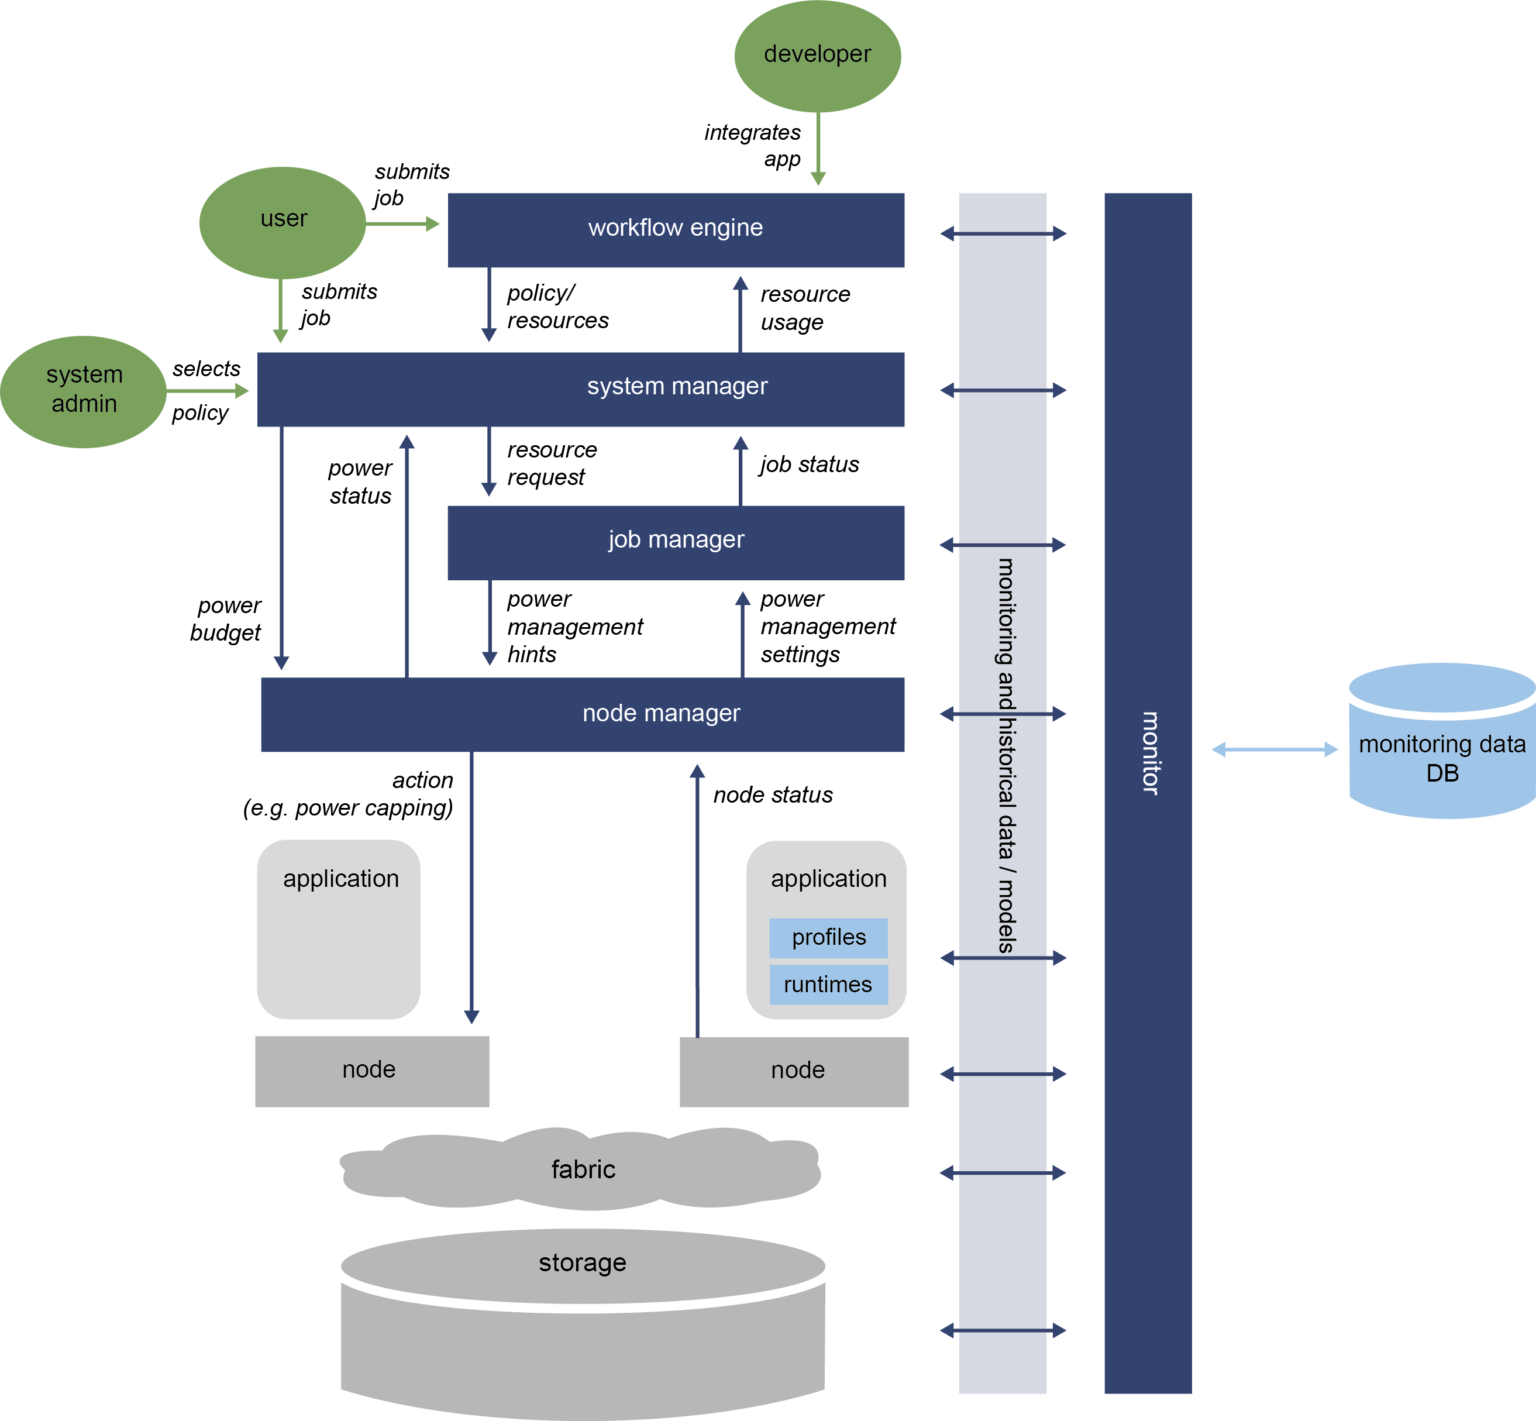
\includegraphics[width=\textwidth]{img/REGALE-Architecture-1536x1421.png}
\end{figure}
% slide 3-4 presentazione
\section{Componenti PowerStack}
\subsection{Workflow engine}
The workflow engine analyses the dependencies and resource requirements of each workflow and decides on how to break the workflow into specific jobs that will be fed to the system manager. 

Job schedulers allow high-performance computing users to efficiently share the computing resources that comprise an HPC system. Users submit batch jobs into one or more batch queues that are defined within the job scheduler. The job scheduler examines the overall set of pending work waiting to run on the computer and makes decisions about which jobs to place next onto the computational nodes within the computer. Generally speaking, the job scheduler attempts to optimize some characteristic such as overall system utilization or fast access to resources for some subset of batch jobs within the computing center's overall workload. The various queues that are defined within the job scheduler may be designated as having higher or lower priorities and may be restricted to some subset of the center's users, thus allowing the job scheduler to understand distinctions of importance of certain jobs within the overall workflow.


\subsection{System Manager}
Receives as input a set of jobs to be scheduled within the system and indicatively decides upon when to schedule each job, to which specific compute nodes to map it, and under which power budget or setting. For this, it constantly monitors and records power and energy telemetry data, and controls power budgets/settings and/or user fairness
%To carry out its work, a job scheduler typically interacts with one or more resource managers. A resource manager is a piece of system software that has privileged ability to control various resources within a datacenter. These resources can include things such as the physical nodes that make up a highperformance computer's computational resources; disks, disk channels, or burst buffer hardware that comprise I/O resources; or network interfaces, network channels, or switches that comprise interconnect resources. For example, a job scheduler might use resource management software to configure the processing cores, memory, disk, and networking resources within one or more computational nodes in accordance with the requested resources for a specific batch job prior to launching that job onto the allocated computational nodes. Finally, in some cases, resource management software might have the ability to actuate pieces of the physical plant that are responsible for delivering electricity to the datacenter or cooling the datacenter

\subsection{Job Manager}
By analysing the profiles, Job Manager decides the target power management knob (CPU power cap, CPU clock frequency scaling or any others) as well as performs code tuning as an option. 

\subsection{Node Manager}
The node manager provides access to node-level hardware controls and monitors. Moreover, the node manager implements processor level and node level power management policies, as well as preserving the power integrity, security and safety of the node. 

\subsection{Monitor}
The monitor is responsible for collecting in-band and out-of-band data for performance, resource utilization, status, power, energy, with minimal footprint, collecting, aggregating, and analysing various metrics, and pushing necessary real-time data to the other entities.
